\section{Value Patterns}
\subsection{1. System Analysis (OOA)}
\subsubsection{Individuals}
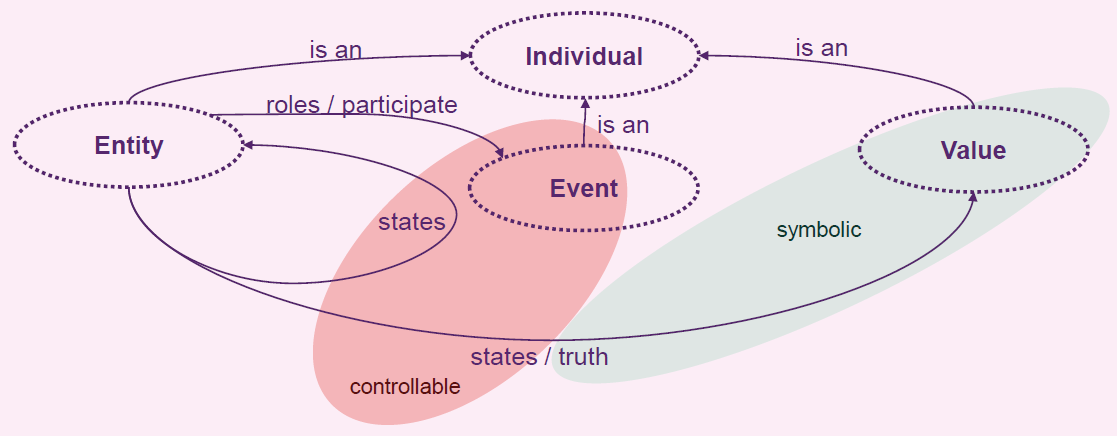
\includegraphics[width=\linewidth]{value_overview.png}

Ein Individual ist etwas, das namentlich benannt und sich zuverlässig von anderen
Individuals unterscheiden kann. \\

\textbf{Events}

Ist ein Individuelles Ereignis. Findet zu einer bestimmten Zeit statt (Bsp. User-Action). \\

\textbf{Entities}

Besteht über die Zeit und kann die Properties oder den State ändern. Entities können Events initiieren (Bsp. Person) \\

\textbf{Values}

Ist ein immaterielles Individual (nicht greifbar), welches ausserhalb von Zeit und Raum existiert (Bsp. Körpergrösse), Not subject to change

\subsection{2. Software Design (OOD)}
\subsubsection{Categories of Objects}
\textbf{Entity}

Drücken Systeminformationen aus, normalerweise persistent, die Identität ist wichtig, um Entity Objects zu unterscheiden (Bsp. User Klasse)\\

\textbf{Service}

Stellen Systemaktivitäten dar, unterscheiden sich durch ihr Verhalten und nicht durch ihren Zustand (Bsp. User Service) \\

\textbf{Value}

Der interpretierte Inhalt ist das dominante Merkmal, ist vergänglich und hat keine signifikante dauerhafte Identität (Bsp. Feld Alter, welches als Integer abgebildet wird) \\

\textbf{Task}

Stellen Systemaktivitäten dar, Haben ein Element der Identität und Zustand

\vfill\null

\subsection{3. Values in Programming (OOP)}

\begin{itemize}
    \item Values werden als Typ dargestellt
    \item Values haben keine Identität (Transparent, Transient Identity)
    \item Funktionen map / konvertieren Werte
    \item Fügt einem primitiven Wert einen Typ hinzu
    \item OO Sprachen müssen Werte oft mit Objekt-Klassen nachahmen (= Value Object Patterns)
    \item Bsp. IBAN Type Object (10 digits, checksum), Klasse Datum wird durch 3 ints dargestellt
\end{itemize}

\subsubsection{Object Aspects}
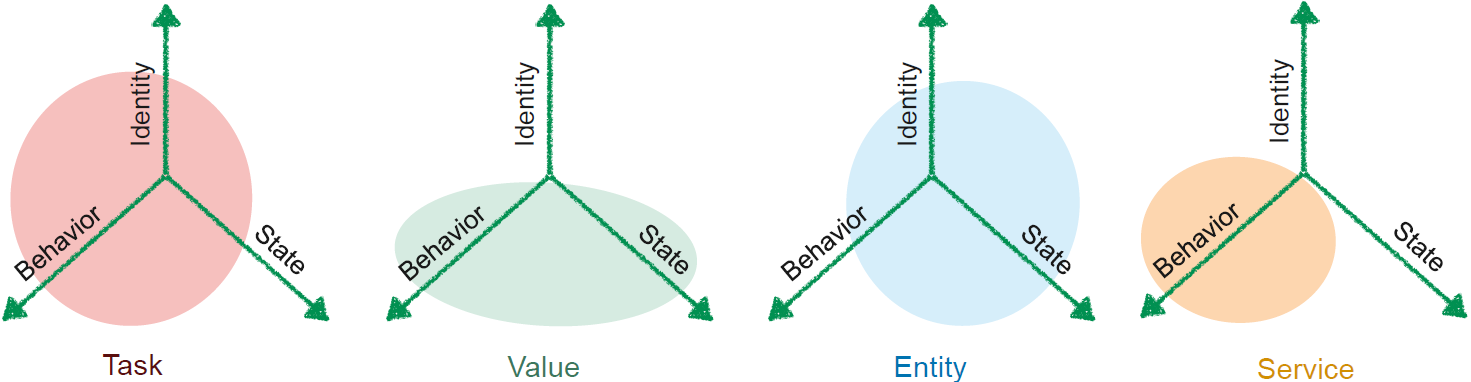
\includegraphics[width=\linewidth]{object_aspects.png}

\begin{itemize}
    \item \textcolor{blue}{Identity} Identität vergänglich oder bedeutsam
    \item \textcolor{blue}{State} Objekt Stateful oder Stateless
    \item \textcolor{blue}{Behavior} Hat das Objekt ein signifikantes Verhalten unabhängig vom State?
\end{itemize}

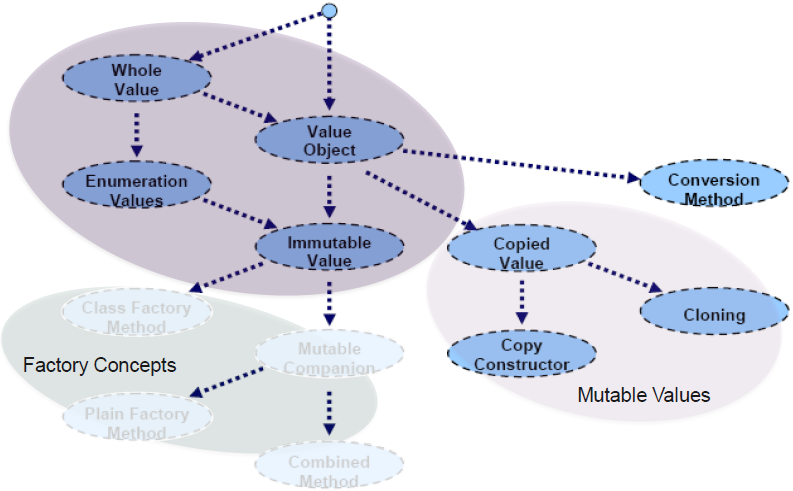
\includegraphics[width=0.8\linewidth]{value_pattern_overview.png}

\subsection{Whole Value}
\subsubsection{Problem}
\begin{itemize}
    \item Plain integers and floating-point numbers are not very useful as domain values
    \item Errors in dimension and intent communication should be addressed at compile time
    \item How can you represent primitive quantities from your problem domain without loss of meaning?
\end{itemize}

\subsubsection{Intention}

Wie können Sie primitive Grössen aus ihrem Problembereich ohne Bedeutungsverlust darstellen?

\subsubsection{Solution}
Drücke den Type der Anzahl als Value Class dar. Also es soll in der Methode \textcolor{red}{nicht} \textit{Date(int year, int month, int day)} sein!\\

\begin{itemize}
    \item Ersetzt den Bedeutungsverlust und die Überprüfung durch eine \textcolor{blue}{dimension} und \textcolor{blue}{range}
    \item \textcolor{blue}{Umfasst einfache Typen oder Attributstypen}
    \item Erlaube keine Vererbung, um Slicing zu vermeiden
    \item Bsp. Year, Month, Day Classes for Dates
\end{itemize}
\begin{lstlisting}
public final class Date {
    public Date(Year year, Month month, Day day) { ... }
}
Date first = new Date(new Year(year), new Month(month), new Day(day));
\end{lstlisting}

\subsection{Value Object / Value Class}
\subsubsection{Problem}

Vergleiche, Indexing und Sortierung sollte nicht auf der Identität, sondern den Inhalt des Value-Objekts adressieren


\subsubsection{Solution}
Überschreibe Methoden, deren Aktion sicht auf den Inhalt und nicht auf die Identität beziehen sollen und implementiere \textcolor{blue}{Serializable}

Override Object's methods who define equality \\

\textbf{Java}
\begin{itemize}
    \item \textit{equals(Object other)}
    \item \textit{hashCode()}
    \item implementiere \textit{Serializable / toString()} if appropriate
\end{itemize}
\vspace{10pt}
\textbf{TypeScript}
\begin{itemize}
    \item \textit{equals(other: Object)}
    \item implementiere \textit{toString()} if appropriate
\end{itemize}

\subsection{Conversion Method}

Value-Objekt sind oftmals verwandt, können aber nicht direkt ohne conversion verwendet werden

\subsubsection{Problem}
\begin{itemize}
    \item Values are strongely informational objects without a role for separate identity
    \item Often Value Objects are somehow related but cannot be used directly without conversion
    \item How could you use different, related Value Objects together without depending on underlying primitive type?
\end{itemize}

\subsubsection{Solution}
Bereitstellung von Typkonvertierungsmethoden, die für die Umwandlung von Wertobjekten in verwandte Formate verantwortlich sind.

\begin{itemize}
    \item Biete einen \textcolor{blue}{Konstruktor}, welcher zwischen den Typen convertiert \\
    $\rightarrow$ \textit{String(char[] value)}
    \begin{itemize}
        \item Keine zusätzliche Methoden Aufrufe nötig
        \item Am intuitivsten, wenn von generischerem Typ zum aktuellen Typ convertiert wird
    \end{itemize}
    \item Eine \textcolor{blue}{Conversion instance Method} convertiert von einem Benutzer definierten Typen zu einem anderen Typen $\rightarrow$ dafür wird eine \textit{toO-therType()-Method} \\
    $\rightarrow$ \textit{Date.toOtherType()}
    \item Erstelle eine \textcolor{blue}{Class Factory Method} mit Conversion charakteristiken $\rightarrow$ Umgekehrte Beziehung mit \textit{toOtherType()}-Methode \\
    $\rightarrow$ \textit{Date.from(Instant i)}
\end{itemize}

\vfill\null
\columnbreak

\subsection{Immutable Value}

Verhindere Probleme, wenn Value-Objekte geteilt werden.

\subsubsection{Problem}
\begin{itemize}
    \item A value exists outside time and space and is not subject to change
    \item Avoid side effect problems when sharing Value Objects
    \item Sharing values across Threads requires thread safety
    \item Values are often threaded as key for associative tables
    \item How can you share Value Objects and guarantee no side effect problems?
\end{itemize}
\subsubsection{Solution}
Setze den internen Zustand des Value Class Objekts beim Konstruktor und erlaube keine Modifikationen

\begin{itemize}
    \item Setze den internal State im Konstruktor und deklariere alle Felder \textit{private final} $\rightarrow$ Klasse als \textit{final} deklarieren und es wird keine Synchronisation benötigt
    \item Ergänzende Techniken $\rightarrow$ \textit{Mutable Companion} und \textit{Class Factory Methods}
\end{itemize}

\subsection{Enumeration Values}
Fixe Range von Values sollte typisiert sein

\subsubsection{Problem}
\begin{itemize}
    \item A fixed range of values should be typed \textit{e.g. months}
    \item Using just int constants doesn't help
    \item Whole Value is only half the solution; range should be constant
    \item How can you represent a fixed set of constant values and preserve type safety?
\end{itemize}
\subsubsection{Solution}
Behandle jede Konstante als ein Whole-Value Instanz, indem sie als \textit{public} deklariert wird
\begin{itemize}
    \item Implementiere eine \textit{Whole Value} und deklariere die \textit{Enumeration-Values} als public read-only fields
    \item Verhindere versehentliches ändern der Konstanten $\rightarrow$ müssen Immutable sein und nur von der Whole-Value erstellt werden
    \item Sind ENUM
\end{itemize}

\vfill\null
\columnbreak

\subsection{Copied Value and Cloning}
Values sollen modifizierbar sein, ohne den Ursprung des internal State zu ändern
\subsubsection{Problem}
\begin{itemize}
    \item Values should be modifiable without changing the origins internal state
    \item How can you pass a modifiable Value Object into and out of methods without permitting callers or called methods to affect the original object?
\end{itemize}

\subsubsection{Solution}
Implementiere ein cloneable-Interface, das verwendet werden kann, wann immer ein Value-Objekt zurückgegeben werden muss oder als Parameter verwendet wird

\begin{itemize}
    \item Cloning bedeutet, erstelle eine Kopie der aktuellen Instanz und allen enthaltenen Feldern
    \item \textit{Cloneable}-Interface und \textit{Object.clone()}-Methode
    \item Imitiert call-by-value / return-by-value Verhalten für Value-Typen
    \item Kann zu immense Objekt Creation Overhead führen $\rightarrow$ Cloning ist eine teure Operation
\end{itemize}

\subsection{Copy Constructor}

Innerhalb von Value-Objekten wollen wir oft wissen, was kopiert werden soll

\subsubsection{Problem}
\begin{itemize}
    \item Within Value Objects we often know exactly what to copy
    \item How can objects be copied without the need of implementing a clone method?
\end{itemize}

\subsubsection{Solution}
Biete einen Weg um ein Objekt basierend auf einer anderen Instanz mit dem exakt selben Typen zu konstruieren

\begin{itemize}
    \item Deklariere die Klasse \textit{final} und leite nur vom Objekt ab $\rightarrow$ Verhinderet das verletzen von Class Invariant
    \item Erstelle ein Copy-Constructor, der eine Instanz mit dem selben Typen consumiert $\rightarrow$ Ist zuständig um die benötigten Informationen zu kopieren. Resultiert in weniger Code und möglicher Cloning Optimisierung
\end{itemize}
\begin{lstlisting}
public final class Date {
    public Date(Date other) {
        // ...
        this.year = new Year(other.year);
    }
}
\end{lstlisting}

\vfill\null
\columnbreak

\subsection{Class Factory Method / Simple Factory (Flyweight)}

Construction von Value-Objekte kann teuer sein. Unterschiedliche Konstruktions-Logik wird benötigt, was in sehr vielen Constructoren enden kann

\subsubsection{Problem}
\begin{itemize}
    \item Construction of Value Objects may be expensive
    \item Different construction logic is required which may result in huge amount of constructors
    \item How can you simplify and potentially optimize construction of Value Objects in expressions without introducing new intrusive expressions?
\end{itemize}

\subsubsection{Solution}

Biete eine statische Methode an, die anstelle von üblichen Konstruktoren verwendet wird. Die Methode gibt entweder neu erstellte Value-Objekte oder cached-Objekte zurück

\begin{itemize}
    \item Deklariere eine oder mehrere statische Creation-Methoden in der Klasse $\rightarrow$ Definiere die Konstruktoren \textit{private}, diese werden von der Class Factory Method ausgeführt
    \item Die statische Methode kann auch Caching Mechanismen enthalten
\end{itemize}
\begin{lstlisting}
public final class Year {

    public static Year of(int value) {
        return new Year(value);
    }

    private Year(int value) {
        this.value = value;
    }
}
\end{lstlisting}

\vfill\null
\columnbreak

\subsection{Mutable Companion (Builder)}

Es muss möglich sein, mit Values, z.B. Rechnen zu können

\subsubsection{Problem}
\begin{itemize}
    \item We need to calculate with values \textit{e.g. 15 working days after exam}
    \item How can you simplify complex construction of an immutable value?
\end{itemize}

\subsubsection{Solution}

Implementiere eine Companion-Klasse, welche modifier-Methoden unterstützt und als Factory für \textit{Immutable-Value-Objekte} agiert

\begin{itemize}
    \item Ist ein Factory Object für Immutable Values $\rightarrow$ Adressiert Effizienz und API Usability Issues
    \item Modifiers erlauben kumulative oder komplexe Zustandsänderungen und eine Query-Method, um auf die immutable Values zuzugreifen
    \item Companion ist weder ein Sub-Typ noch ein Super-Type des Immutable Values, also gehört es nicht zur selben Familie
    \item In Kombination mit Companion, wir die Factory \textit{Plain Factory method} genanntFactory Object for immutable values
\end{itemize}
\begin{lstlisting}
public final class YearCompanion {
    private int value;

    public YearCompanion(Year toModify) {
        this.value = toModify.getValue();
    }
    /* modifying methods */
    public void next() { value++; }

    public Year asValue() { /* Factory Method */
        return Year.of(value); }
}
\end{lstlisting}

\subsection{Relative Values}

Value-Objekte werden auf dessen Zustand, nicht dessen Identität verglichen

\subsubsection{Problem}
\begin{itemize}
    \item Value Objects are compared by their state, not their identity
    \item Relative comparison between Value Objects for appropriate values should be provided
    \item How can a Value Obejct be compared against others in a typed way?
\end{itemize}
\subsubsection{Solution}
Implementiere den Vergleich von \textit{Value Objects}, indem das \textit{Comparable}-Interface implementiert wird

\begin{itemize}
    \item \textcolor{blue}{Override-Overload Method Pair} \textit{Comparable$<$?$>$} und \textit{equals(? other)} soll als paar überschrieben werden
    \item \textcolor{blue}{Type$<$T$>$ spezifische Overload} Implementiere \textit{Comparable$<$T$>$.compareTo(T other)} und \textit{equals(T other)} für den aktuellen \textit{Typ$<$T$>$}. Für andere Value Object Typen erstelle eine Comparator-Klasse die das \textit{Comparator$<$TOther$>$} Interface implementiert
    \item Erstelle eine \textcolor{blue}{Bridge-Methode} für \textit{equals(Object other)} und leite es weiter zu \textit{equals(T other)}
\end{itemize}

\columnbreak

\subsection{Discussion}
\textbf{Difference between Whole Value and Immutable Value}
\begin{itemize}
    \item \textcolor{blue}{Whole Value} Value with a unit should be encapsulated in a class
    \item \textcolor{blue}{Immutable Value} Value within an object must be immutable
\end{itemize}
\vspace{10pt}
\textbf{When would you prefer Class Factory Method over a conversion constructor?}
\begin{itemize}
    \item \textcolor{blue}{Factory} A foreign value type should be converted into the current value format
    \item \textcolor{blue}{Contructor} A more generic type should be converted into the current type
\end{itemize}
\vspace{10pt}
\textbf{What are the most important liabilities of the Mutable Value concept?}

Concept of Cloning / Copied Value may be missed by the programmer which results in to hard to find errors

